%%
%% This is file `sample-sigconf.tex',
%% generated with the docstrip utility.
%%
%% The original source files were:
%%
%% samples.dtx  (with options: `sigconf')
%% 
%% IMPORTANT NOTICE:
%% 
%% For the copyright see the source file.
%% 
%% Any modified versions of this file must be renamed
%% with new filenames distinct from sample-sigconf.tex.
%% 
%% For distribution of the original source see the terms
%% for copying and modification in the file samples.dtx.
%% 
%% This generated file may be distributed as long as the
%% original source files, as listed above, are part of the
%% same distribution. (The sources need not necessarily be
%% in the same archive or directory.)
%%
%% The first command in your LaTeX source must be the \documentclass command.
\documentclass[sigconf]{acmart}

%%%% As of March 2017, [siggraph] is no longer used. Please use sigconf (above) for SIGGRAPH conferences.

%%%% Proceedings format for SIGPLAN conferences 
% \documentclass[sigplan, anonymous, review]{acmart}

%%%% Proceedings format for SIGCHI conferences
% \documentclass[sigchi, review]{acmart}

%%%% To use the SIGCHI extended abstract template, please visit
% https://www.overleaf.com/read/zzzfqvkmrfzn

%%
%% \BibTeX command to typeset BibTeX logo in the docs
\AtBeginDocument{%
  \providecommand\BibTeX{{%
    \normalfont B\kern-0.5em{\scshape i\kern-0.25em b}\kern-0.8em\TeX}}}

%% Rights management information.  This information is sent to you
%% when you complete the rights form.  These commands have SAMPLE
%% values in them; it is your responsibility as an author to replace
%% the commands and values with those provided to you when you
%% complete the rights form.
% \setcopyright{acmcopyright}
% \copyrightyear{2021}
% \acmYear{2021}
% \acmDOI{10.1145/1122445.1122456}

%% These commands are for a PROCEEDINGS abstract or paper.
 %\acmConference[Woodstock '18]{Woodstock '18: ACM Symposium on Neural
 %  Gaze Detection}{June 03--05, 2018}{Woodstock, NY}
% \acmBooktitle{Woodstock '18: ACM Symposium on Neural Gaze Detection,
 %  June 03--05, 2018, Woodstock, NY}
% \acmPrice{15.00}
 %\acmISBN{978-1-4503-9999-9/18/06}


%%
%% Submission ID.
%% Use this when submitting an article to a sponsored event. You'll
%% receive a unique submission ID from the organizers
%% of the event, and this ID should be used as the parameter to this command.
%%\acmSubmissionID{123-A56-BU3}

%%
%% The majority of ACM publications use numbered citations and
%% references.  The command \citestyle{authoryear} switches to the
%% "author year" style.
%%
%% If you are preparing content for an event
%% sponsored by ACM SIGGRAPH, you must use the "author year" style of
%% citations and references.
%% Uncommenting
%% the next command will enable that style.
%%\citestyle{acmauthoryear}

%%
%% end of the preamble, start of the body of the document source.
\begin{document}

\title{RNA\_LZW: A Novel Method for Detection of Stems and Pseudoknotted Structures in Non-Coding RNA}

\author{Claire Champernowne}
\email{cchampernowne@gmail.com}
\affiliation{%
  \institution{University of Victoria}
}

\author{Quinn Gieseke}
\email{qgieseke@gmail.com}
\affiliation{%
  \institution{University of Victoria}
}

\renewcommand{\shortauthors}{Champernowne and Gieseke, et al.}

\begin{abstract}
  A clear and well-documented \LaTeX\ document is presented as an
  article formatted for publication by ACM in a conference proceedings
  or journal publication. Based on the ``acmart'' document class, this
  article presents and explains many of the common variations, as well
  as many of the formatting elements an author may use in the
  preparation of the documentation of their work.
\end{abstract}

%%
%% Keywords. The author(s) should pick words that accurately describe
%% the work being presented. Separate the keywords with commas.
\keywords{pseudoknot, non-coding RNA, secondary structure, tertiary structure, dot-bracket notation}

\maketitle

\section{Introduction}
Detecting RNA secondary structures is a process which is integral to understanding the functions of non-coding RNA sequences. Though there are existing bioinformatics tools used for detection, these programs are not without their limitations. \\
Specifically, RNAz uses a sliding window approach in its analysis of a sequence [1], [2], meaning there may be structures with loops existing outside the scope of the window.\\
The Lempel-Ziv-Welch (LZW) algorithm is a universal lossless compression algorithm used for a variety of applications such as Unix file compression. The algorithm compresses data by using a dictionary to assign common sequences of characters to a fixed-length code (typically 12-bit) [3].\\
Because RNA structure exists in a 3-dimensional capacity, with its final form assuming a tertiary structure, base pairings which may appear to be distant from one another in a secondary structure can in reality exist very closely to one another once their tertiary structure is assumed. Given the LZW algorithm’s dictionary approach to pattern-matching,  RNA\_LZW can detect the presence of distant pseudoknots in a structure in much the same way that it detects regular base pairing. \\
We propose that RNA\_LZW could serve as a pre-processing step to determine if there are notable base pairings throughout a given sequence, which may not be accounted for by standard secondary structure detection methods.

\section{algorithms}


\subsection{Lempel-Ziv-Welch Encoding}

RNA\_LZW uses only the encoding step of the LZW compression algorithm.  A high level overview of the encoding portion of the LZW algorithm as employed in RNA\_LZW is shown below:

\begin{enumerate}
\item Initialize the dictionary to contain all keys of length one. 
	\begin{enumerate}
		\item In this case, the dictionary initially contains only four characters; A,U,C, and G. 
	\end{enumerate}
\item Initialize a buffer as the first character in the sequence.
\item Add characters from the sequence to the buffer until the buffer represents a key that is not already represented in the dictionary. Once the buffer is added to the dictionary as a key, it is reset to just the last character.
	\begin{enumerate}
		\item Though not represented in a normal LZW algorithm, RNZ\_LZW records additional metadata about the position of the buffer in the greater sequence into the dictionary.
	\end{enumerate}
\item Though LZW encoding normally cannot iterate multiple times due to its need to be decoded without the dictionary; RNA\_LZW acts with global information, and does not have that restriction, and therefore uses multiple iterations to build a much more robust dictionary.
\end{enumerate}


\subsection{Dot-Bracket Construction}
Once we have the dictionary with many possible base matches, we must remove overlapping matches, and place only the most likely ones into the final output. Currently we measure stem likelihood first by length, and then by distance. The steps are as follows:
\begin{enumerate}
\item Remove impossible matches.
	\begin{enumerate}
	\item While adding entries to the dictionary, it is possible to add overlapping matches, where a sequence of bases can be paired with itself. For example, the sequence \texttt{UGAUAGCA} when reversed will exactly pair to itself. 
	\end{enumerate}
\item For each dictionary entry, parse the possible match locations and select the pair of base sequences that are the shortest distance apart.
\item Sort by match length.
\item Check the location of each stem placement in the output:
	\begin{enumerate}
	\item If the location is empty, add the stem to the output, marked by a unique key at every base location along the stem
	\item If any base in the location already has a stem, skip. Since we iterate from longest stems down to shortest, this biases the algorithm towards including longer stems.
	\end{enumerate}
\end{enumerate}
At this point in the algorithm, the output consists of a unique symbol per stem (The index in the output of the start of the right stem half), that is replicated at each base in the stem. To convert into standard dot-bracket notation, we must essentially reduce the number of bracket symbols down. For the purposes of notating pseudoknots, we use the bracket progression of \texttt{([\{<ABCD} for opening brackets, and \texttt{dcba>\}])} for closing braces.
This algorithm utilizes a single modified stack in order to match braces as it progresses through the output sequence. The stack is allowed to have "transparent" entries that stay on the stack, but peek and pop operations will return the first non-transparent entry on the stack.
\begin{enumerate}
	\item Iterate through the output, left to right.
		\begin{enumerate}
		\item If the current value equals the top of the stack, pop the top of the stack. This is equivalent to finding a normal brace match
		\item If the current value equals the index of the match, and that value is not on top of the stack, then we have a closing bracket with its requisite opening bracket must be beyond the last opening bracket, meaning we have found a pseudoknonot.
			\begin{itemize}
			\item Since representing a pseudoknot requires a new style of brace, we iterate through the stack between the opening and closing brace (including transparent entries), seeking out the highest value of brace. We then assign a one higher value of brace to the current pair, and make both entries transparent. 
			\end{itemize}
		\item If neither of the above cases are true, we have a normal opening brace. Push current value to the stack.
		\end{enumerate}
\end{enumerate}
Finally, we iterate through the output one more time, converting each unique id into its corresponding brace value, and replacing any gaps with '.'.


\section{results}

In order to test for RNA\_LZW's efficacy as a preprocessing(?) step in identifying potentially relevant stems and pseudoknots in a given structure, it was tested using sequences where the secondary structure is known.  All sequences used were sourced from the RNACentral database. The dot-bracket notations of these known sequences were then compared to the dot-bracket output generated by RNA\_LZW.


\subsection{Homo sapiens tRNA-SeC (anticodon TCA) 1-1 (TRU-TCA1-1)}

\begin{figure}
  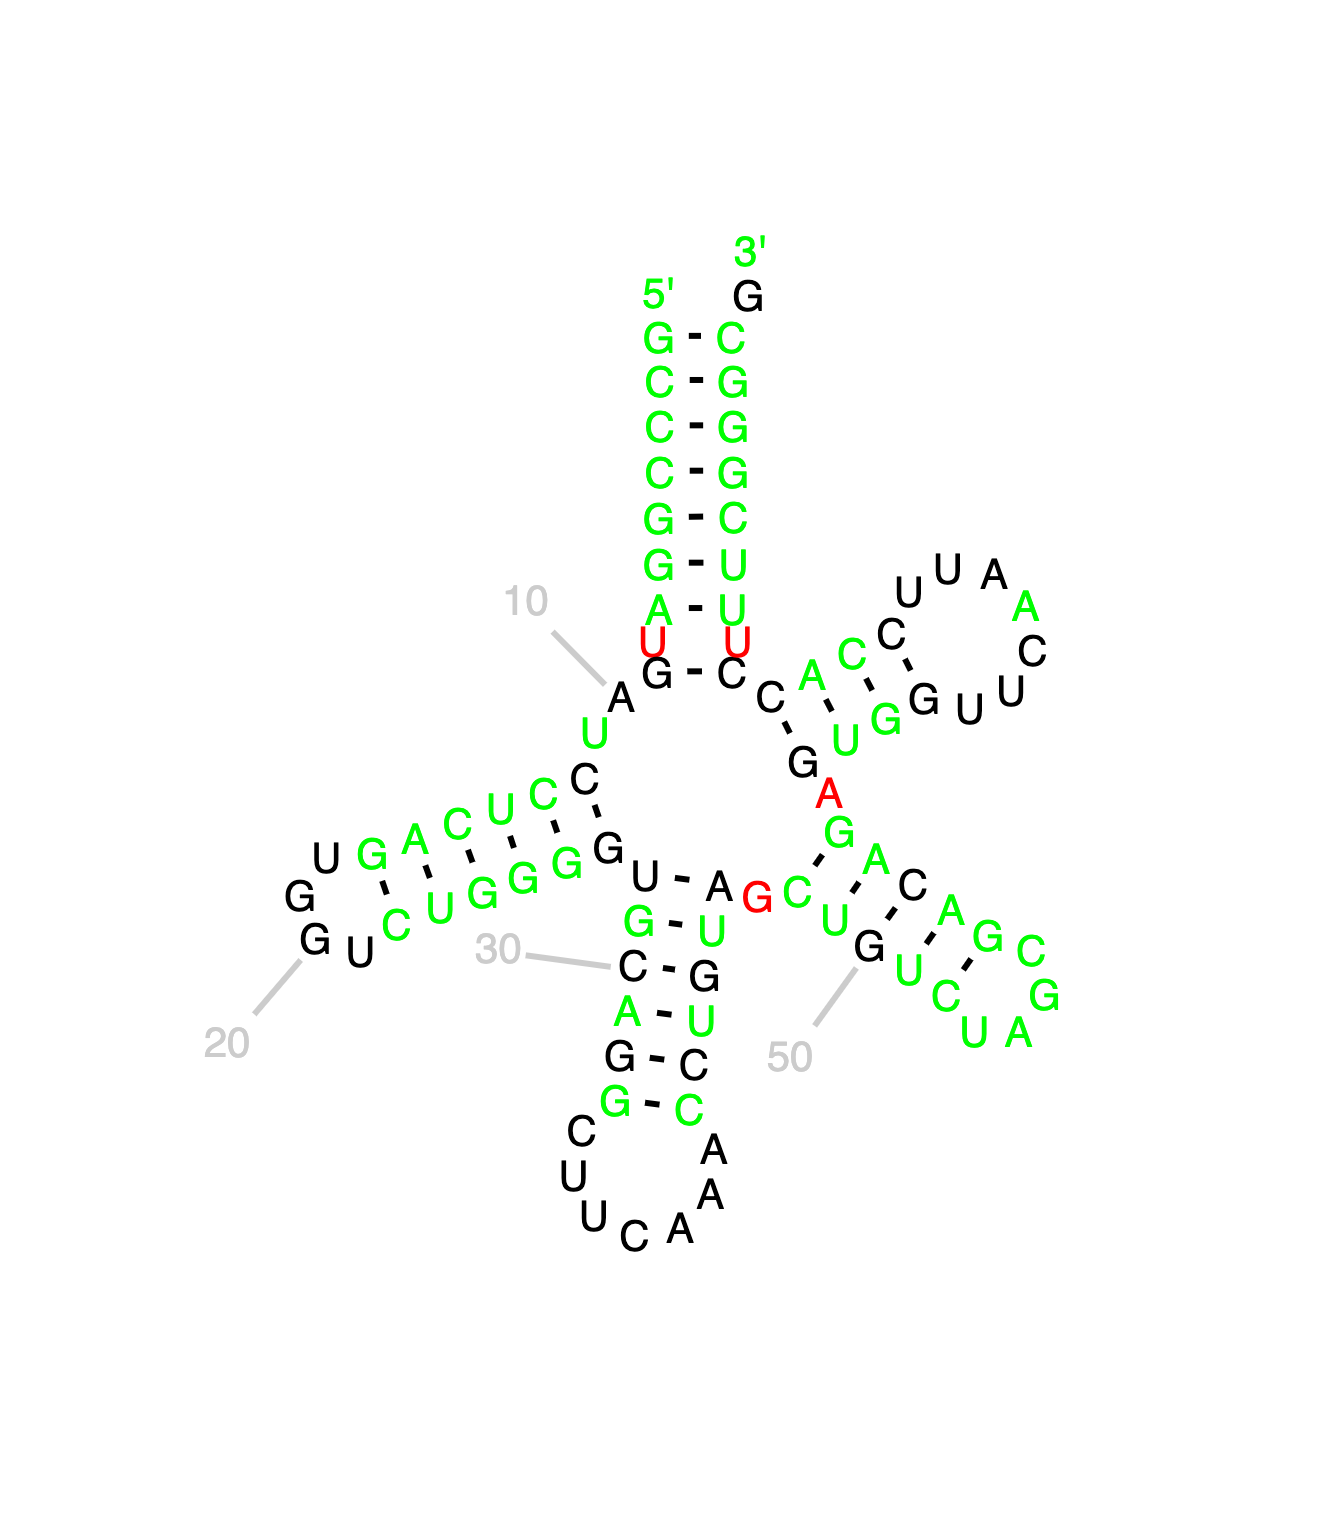
\includegraphics[width=\linewidth]{for_paper1.png}
  \caption{Homo sapiens tRNA-SeC, generated using R2DT secondary structure visualization}
  \label{fig:tRNA}
\end{figure}

As seen in Figure \ref{fig:tRNA},  tRNAs are short sequences which serve as a good benchmark to visualize whether RNA\_LZW is capable of outputting structures that are at all similar to those obtained by tried and true methods of RNA secondary structure discovery. \\
Clearly RNA\_Z cannot serve as a replacement for more accurate methods of secondary structure construction; however, the output in Table \ref{tab:tRNA} shows that RNA\_Z is capable of producing somewhat similar structural features to a known dot-bracket structure.  In the case of this tRNA sequence,  RNA\_Z achieves 71\% accuracy when doing a string comparison to the known dot-bracket structure. \\
Due to the small size of this sequence, RNA\_Z's output is clearly different from the known structure, but the hypothesis that RNA\_Z is capable of matching base pairs from any range in the structure, is supported by the output generated from this sequence. 

\begin{table}
  \caption{Dot-Bracket Comparison}
  \label{tab:tRNA}
  \begin{tabular}{l}
    \textbf{Sequence}\\
    GCCCGGAUGAUCCUCAGUGGUCUGGGGUGCAGGCUUCA\\
    AACCUGUAGCUGUCUAGCGACAGAGUGGUUCAAUUCCA\\
    CCUUUCGGGCG\\
    \midrule
    \textbf{RNA\_LZW Output}\\
	(((((..(((...))).............((((....((())))...(((((....))))).((((.......)))).)))))))).\\
    \midrule 
    \textbf{Known Dot-Bracket Structure}\\
    (((((((.(..((((((....))))))((((((.......)))))).(((((....))))).((((.......))))).))))))).\\
\end{tabular}
\end{table}


\subsection{Homo sapiens telomerase RNA}

Telomerase is a ribonucleoprotein, meaning that it is a complex structure comprised of non-coding RNA and a protein binding to one another. Telomerase RNA contains a pseudoknot which is integral to telomerase's function [5].  Figure \ref{fig:telomerase} helps visualize how these pseudoknots appear in nature.\\
Though the length of the sequence (450 nucleotides) means that visual comparison shown in Table \ref{tab:telomerase} is difficult for the reader to assess. When doing a comparison of string similarity, RNA\_Z achieves 51\% accuracy.

\begin{figure}
  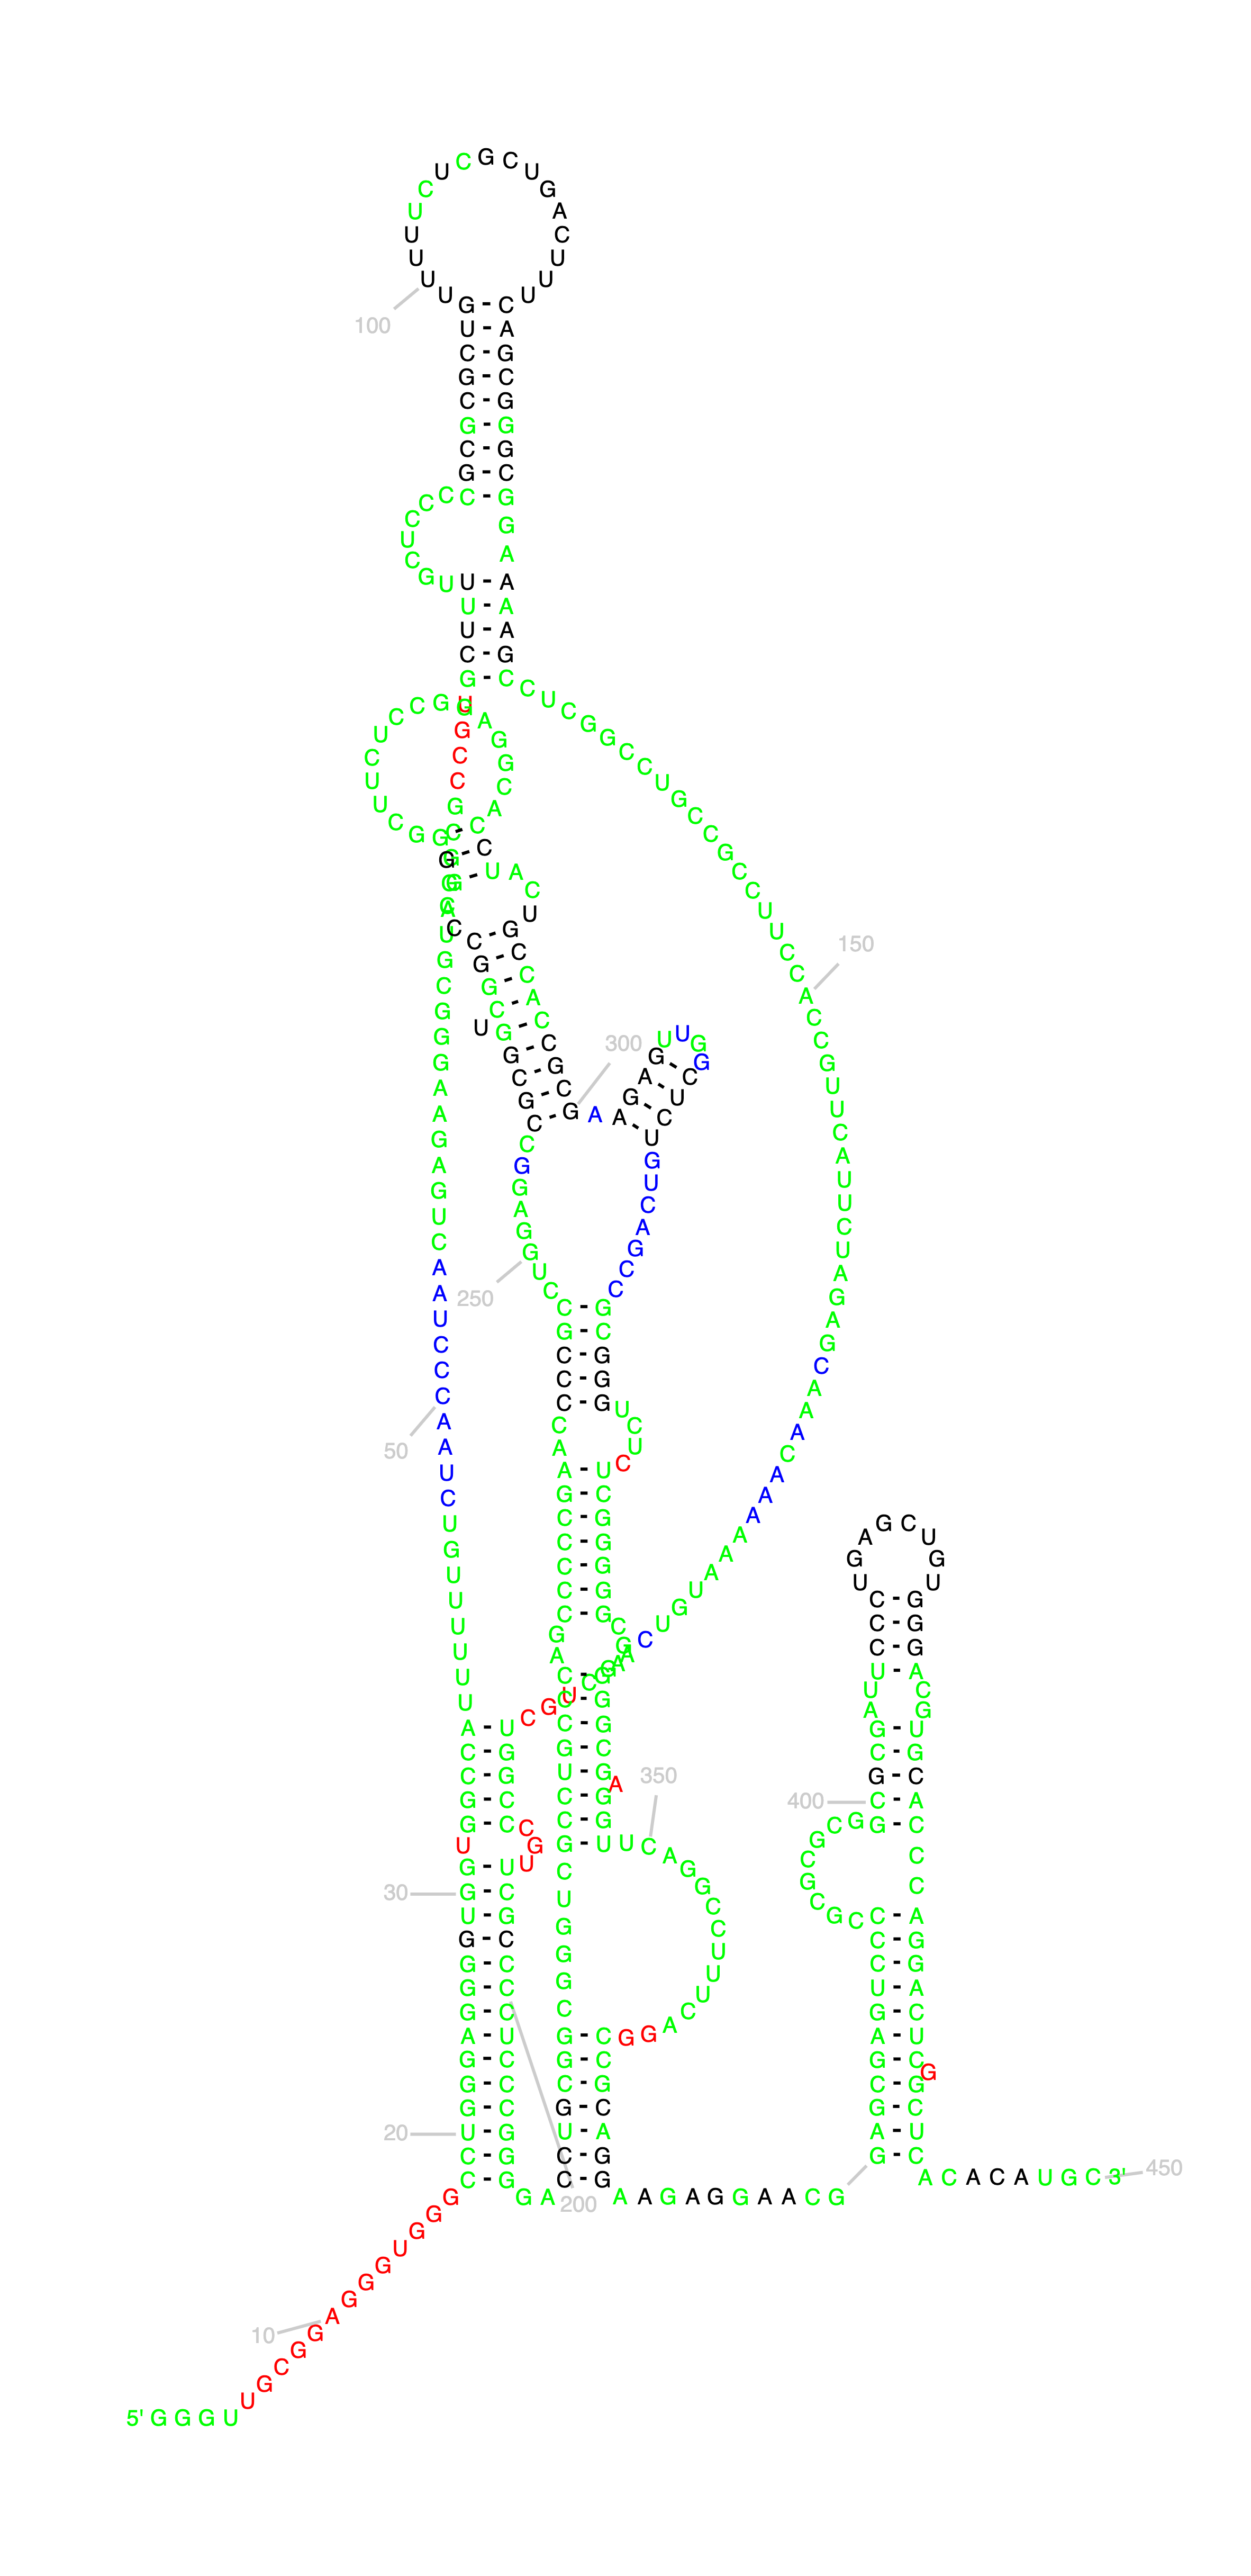
\includegraphics[width=\linewidth]{for_paper.png}
  \caption{Homo sapiens telomerase RNA, generated using R2DT secondary structure visualization}
  \label{fig:telomerase}
\end{figure}

\begin{table}
  \caption{Dot-Bracket Comparison}
  \label{tab:telomerase}
  \begin{tabular}{l}
    \textbf{Sequence}\\
    \midrule
    \textbf{RNA\_LZW Output}\\
    (((((........(((((...(((((((.((((((.(((((((((..))))).....((((((.....(((((.......(((((((.((((((((...\\
    (((((.((((((...))))))....))))).....((((((.)))))................)))))))))))))))..((((.))))..((((((.))\\
    )))))....((((((((((..)))....)))))((((((((.(((((........((((((......))))))))))).......((((...))))))\\
    ....((((....)))).....)))))).....)))))))).......)))).))))))..((((())))))).....))))))..(((((((..))))))))\\
    ........)))))....((((..((()))))))))))))............\\
    \midrule 
    \textbf{Known Dot-Bracket Structure}\\
    .................((((((((((((((.(((((........................................(((((.......(((((((((..............\\
    ...)))))))))..))))).......................................................)))))...))))))))))))))..(((((((......\\
    ((((((((..(((((((..(((((........(((((.((((..(((...............)))...))))))))).((((....)))).......)))))....\\
    )))))))...))))).)))..............)))))))..........(((((((((((........(((((..((((........))))..)))))..)))))))\\
    .))))........
\end{tabular}
\end{table}

\subsection{Homo sapiens RNA, 28S ribosomal N1 (RNA28SN1)}

Ribosomal ribonucleic acid is a primary component of ribosomes which carries out protein synthesis. Thus, rRNA is a prime candidate for testing of larger sequences (5,066 nucleotides). 
In doing a string comparison, RNA\_LZW only achieved 38\% accuracy when analyzed against the known secondary structure. 

\begin{figure}
  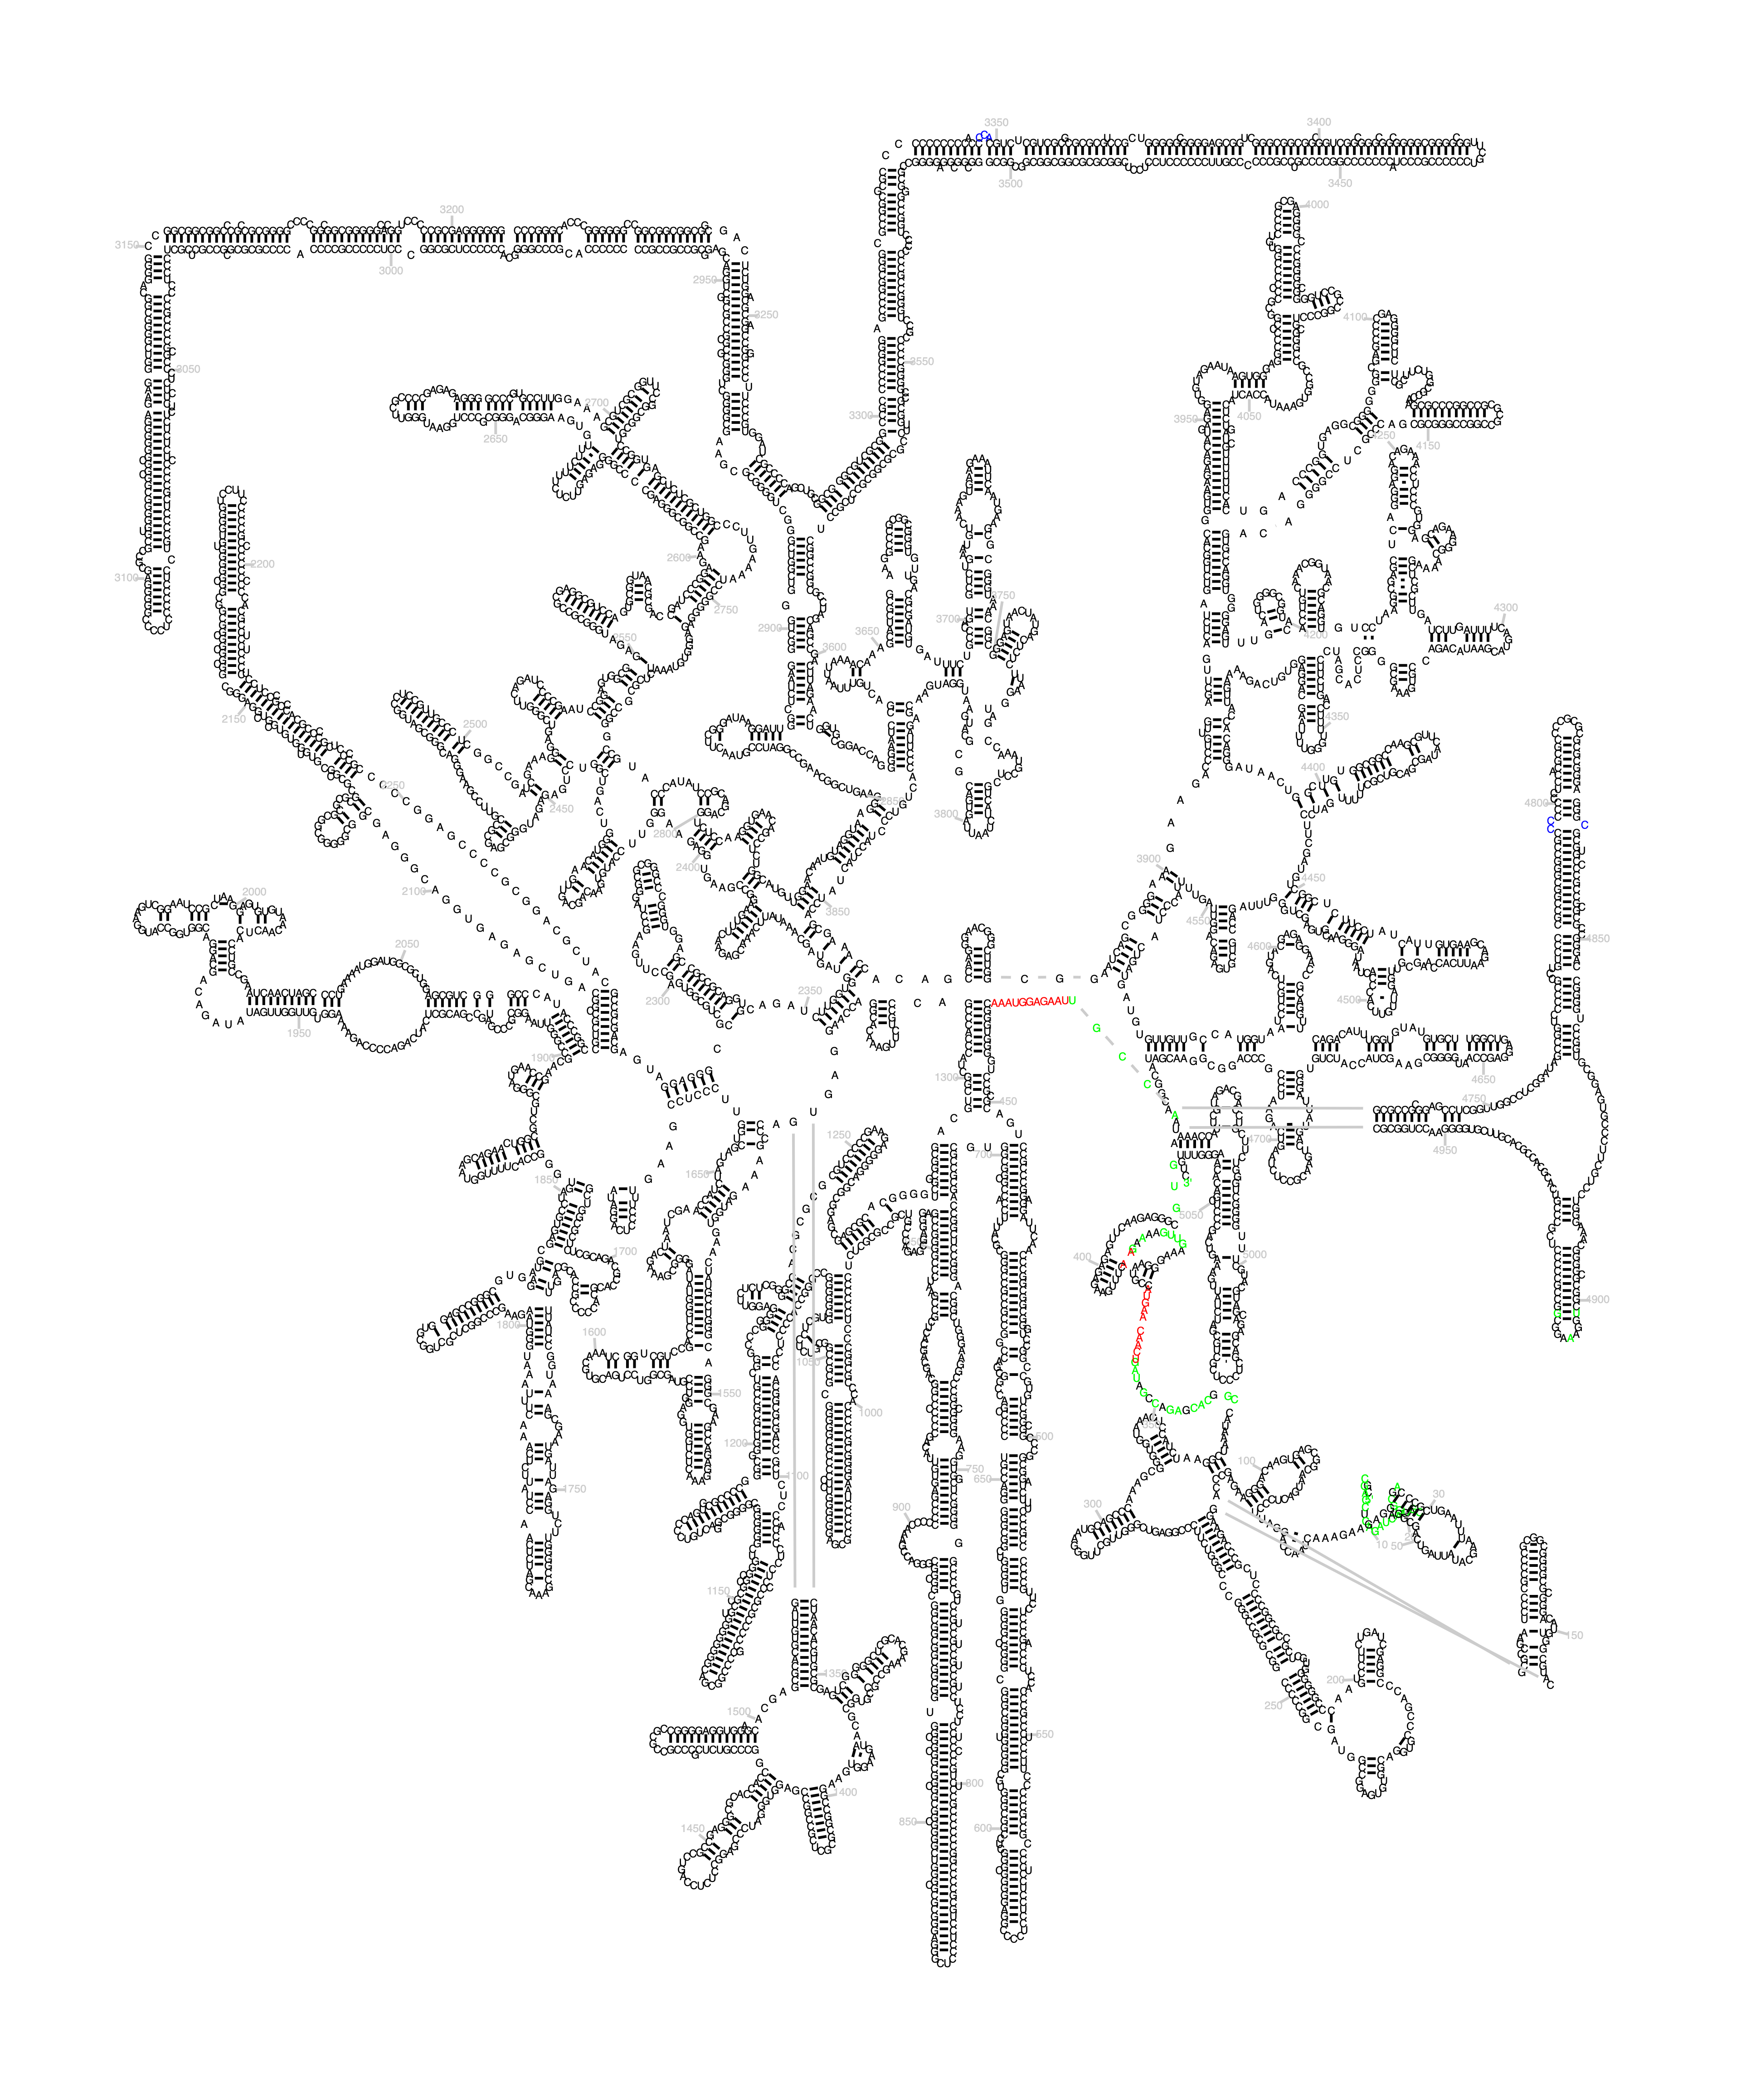
\includegraphics[width=\linewidth]{for_paper2.png}
  \caption{Homo sapiens 28S ribosomal RNA, generated using R2DT secondary structure visualization}
  \label{fig:ribosomal}
\end{figure}

\section{discussion}

heyo\\

\section{conclusion}

The title of your work should use capital letters appropriately -
\url{https://capitalizemytitle.com/} has useful rules for
capitalization. Use the {\verb|title|} command to define the title of
your work. If your work has a subtitle, define it with the
{\verb|subtitle|} command.  Do not insert line breaks in your title.

If your title is lengthy, you must define a short version to be used
in the page headers, to prevent overlapping text. The \verb|title|
command has a ``short title'' parameter:
\begin{verbatim}
  \title[short title]{full title}
\end{verbatim}

\section{bibliography}

[1] A. R. Gruber S. Findeiß, S. Washietl, I. L. Hofacker, and P. F. Stadler, “RNAZ 2.0: Improved Noncoding RNA Detection,” Pacific Symposium on Biocomputing, pp. 69–79, 2010. 

[2] S. Washietl, I. L. Hofacker, and P. F. Stadler, “Fast and Reliable Prediction of Noncoding RNAs,” Proceedings of the National Academy of Sciences, vol. 102 (7), pp. 2454–2459, 2005.  

[3] T. A. Welch, "A Technique for High-Performance Data Compression," in Computer, vol. 17, no. 6, pp. 8-19, June 1984, doi: 10.1109/MC.1984.1659158.

[4] I. L. Hofacker, S. Bonhoeffer, P. F. Stadler, R. Lorenz, and W. Fontana, “RNAfold manual page for RNAfold 2.4.16,” Theoretical Biochemistry Group. [Online]. Available: \url{https://www.tbi.univie.ac.at/RNA/RNAfold.1.html#heading7}. [Accessed: 21-Feb-2021]. 

[5] https://www.ncbi.nlm.nih.gov/pmc/articles/PMC21964/


\end{document}
\endinput
%%
%% End of file `sample-sigconf.tex'.
